\documentclass[12pt]{article}
\usepackage[margin=1in]{geometry}
\usepackage{graphicx}
\usepackage{amsmath, amsthm, amssymb, latexsym}
\usepackage{enumerate}
\usepackage{color}
\newtheorem*{defn}{Definition}
\begin{document}
\title{Mid-semester report\\ 
Interactive Visualizations in Mathematica 
\\
Spring 2021}
\author{Faculty Mentor: A.J. Hildebrand \\
    Project Leader: Efstathios Konstantinos Chrontsios Garitsis \\
	IGL Scholars: Xiaojun Jia, Adithya Swaminathan, \\
	Dimitrios Tambakos, Troy Yang, Sarah Zimmerman}
	\date{March 22, 2021}
\maketitle
\section{Project Goals}
We split into two subgroups in order to create fractal-like visualizations derived by different aspects of math. The first subgroup concentrates on  Julia sets of complex cubic \mbox{polynomials} and tries to identify patterns within their fractal-like visualizations while the coefficients of the polynomials change. The second subgroup is investigating the behavior of fractals constructed from sum-of-digit functions.

\section{Julia Sets}
Let $P: \mathbb{C} \rightarrow \mathbb{C}$ be a complex polynomial and ${P^k}$ denote the k-th iterate of ${P}$, i.e., $P^k = P \circ P \circ \dots \circ P$  k times.

\begin{defn}
The \textbf{Julia Set} is defined to be the boundary of the set of all points ${z \in \mathbb{C}}$ for which the set $\{P^{k}(z) : k \in \mathbb{N}\}$ is bounded.
\end{defn}

Our research is focused on how the Julia Sets of polynomials change while the \mbox{coefficients} change. This has been extensively studied for polynomials of the form ${z^2 + c}$ and many \mbox{visualizations} of those Julia sets have been created. We focus on polynomials of the form ${z^3 + az^2 + \lambda z}$ where ${a}$ is a complex number and ${\lambda = e^{2 \pi i \theta}}$ where ${\theta}$ is an irrational number.\\

When $a$ varies among integers and $\theta$ is constant, we noticed that graphs of Julia sets have central symmetry when $a_1=-a_2$. For example, when $\theta = \sqrt{2}$ and $a\in [-2,2] \cap \mathbb{Z}$, the graphs for $a_1 = -1$ and $a_2 = 1$ are central symmetric.
\newpage
\begin{center}
      	~\\$a_1 = -1$ \hspace{2.15in}$a_2 = 1$
        ~\\\includegraphics[
        height=1in,
        width=2in]{sqrt_2_a=-1.PNG}
        \hspace{0.6in}
        \includegraphics[
        height=1in,
        width=2in]{sqrt_2_a=1.PNG}
\end{center}

However, we also came across instances where the graphs of the Julia set do not have central symmetry. For example, fix $\theta = \pi^\pi$ and let $a \in \{0.59+1.5xi \mid x \in \mathbb{Z}\}$. The graphs for $x=-1$ and $x=1$  lose central symmetry, as shown below:
\begin{center}
    ~\\$a=0.59-1.5i$ \hspace{1.25in}$a=0.59+1.5i$ 
    ~\\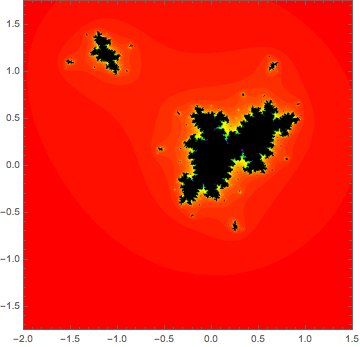
\includegraphics[width=1.25in,height=1.25in]{pi2pi1.png}
    \hspace{1in}
    \includegraphics[width=1.25in,height=1.25in]{pi2pi3.png} 
\end{center}

Last but not least, we are studying the possibility of patterns of the Julia set when ${a}$ is fixed and ${\theta}$ changes among irrational numbers.

\section{Sum-of-Digit Fractals}
Let  $s_{b}(n)$ denote the sum of the digits of a number $n$ in base $b$.
For example, in base $b=10$ we have 
$s_{10}(15) = 1 + 5 = 6$, while in base $b=2$,
 $s_{2}(15) =  1 + 1 + 1+ 1 = 4$ since $15$ has base $2$ representation $1111$.
 We consider the exponential sum
\[ S_{b, p}(N) = \sum_{n=1}^{N}{e^{2\pi i\, s_{b}(n)/p}},
\]
where $s_b(n)$ is the sum-of-digit function and $p$ is a parameter.
Since the terms $e^{2\pi i s_b(n)/p}$ in $S_{b,p}(n)$ are complex numbers, we can interpret them as vectors in the $xy$-plane given by:
\[
e^{2\pi i s_b(n)/p}=(\cos(2\pi  s_{b}(n)/p), \sin(2\pi s_{b}(n)/p))
\]

\begin{defn}Given a base $b$ and a parameter $p$, we define the associated \textbf{sum-of-digit fractal} to be the  curve whose steps are given by the terms of $S_{b,p}(N)$.
\end{defn}

%Figure \ref{fig:five-steps} shows the first 5 steps of the sum-of-digit fractal with $b=2$ and $p=7$.
In the case where $b \equiv 1 \pmod{p}$, we can show that the corresponding fractal is given by a regular $p$-gon, as illustrated in Figure \ref{fig:p-gons}.

For the case where $b \equiv 0 \pmod{p}$, we can obtain a set of $p$ overlapping $p$-gons that share a common vertex in the center, as seen in Figure \ref{fig:multiple-p-gons}.
% , given by Figure \ref{fig:multiple-p-gons}.


% \begin{figure}[htb!]
%     \begin{center}
%         \includegraphics[
%         height=0.25\textheight,
%         width=0.5\textwidth]{arrows_w_axes.png}
%         \end{center}
        
%         \caption{The first 5 steps of the sum-of-digit fractal $S_{2,7}(N)$.}
%         \label{fig:five-steps}
% \end{figure}

\begin{figure}[htb!]

    \begin{center}
    \includegraphics[width=2in,height=1.75in]{pentagon.png} 
    \hspace{0.2in} \includegraphics[width=2in,height=1.75in]{hexagon.png}
    \end{center}
    \caption{Sum-of-digit fractals for $p = 5, b = 6$ (left), and $p = 6, b = 7$ (right).}
    \label{fig:p-gons}
    \end{figure}

\begin{figure}[htb!]
    \begin{center}
    \includegraphics[width=2in,height=1.75in]{bequalsn3.png}
    \hspace{0.2in} \includegraphics[width=2in,height=1.75in]{bequalsn4.png}
    \\
    \includegraphics[width=2in,height=1.75in]{bequalsn5.png}
    \hspace{0.2in} \includegraphics[width=2in,height=1.75in]{bequalsn6.png}
    \end{center}
    \caption{Sum-of-digit fractals for $p = 3, b = 3$ (top left), $p = 4, b = 4$ (top right),
    $p = 5, b = 5$ (lower left), and $p = 6, b = 6$ (lower right).}
    \label{fig:multiple-p-gons}
\end{figure}

\clearpage
For irrational values of $p$, the sum-of-digit fractals can take a great (and largely unpredictable) variety of different shapes  as illustrated in Figure \ref{fig:irrational}. 
\begin{figure}[htb!]
    \begin{center}
    \includegraphics[width=2in,height=1.75in]{sqrt7_irrational.png}
    \hspace{0.2in} \includegraphics[width=2in,height=1.75in]{logpi.png}
    \\
    \includegraphics[width=2in,height=1.75in]{base5_8piover3.png}
    \hspace{0.2in} \includegraphics[width=2in,height=1.75in]{logsqrtpi.png}
    \end{center}
    \caption{Sum-of-digit fractals irrational for $p$ values: $n = 1000$, $p = 2\sqrt{6}$, $b = 7$  (top left), $n = 1000$, $p = \ln(\pi)$, $b = 8$ (top right), $n = 500$, $p = 8\pi/3$, $b = 5$ (bottom left), $n = 1000$, $p = \ln(\sqrt{\pi})$, $b = 10$ (bottom right).}
    \label{fig:irrational}
\end{figure}

\section{Next Steps}

In the coming weeks, we plan to refine the code for these visualizations, add more functionality, and create interactive animations. We also hope to prove or explain some of the observed behavior.


\end{document}